\subsection{Schuhkonstruktion}
\begin{figure}[tb]
	\hfill
	%\centering
	\begin{subfigure}[c]{.49\linewidth}
		\centering
		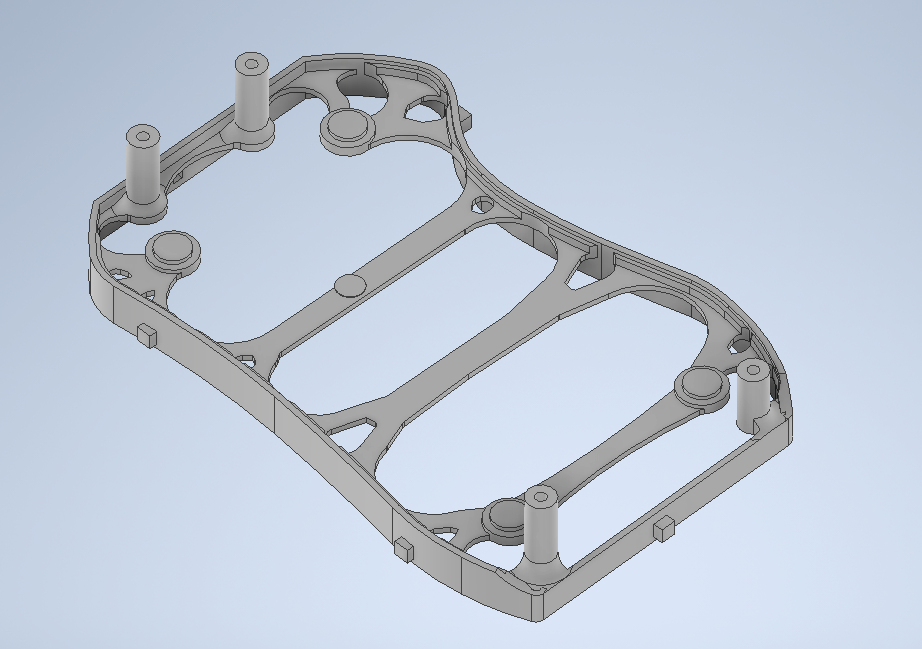
\includegraphics[width=\linewidth]{Bilder/Schuh_oben.png}
	\end{subfigure}
	\begin{subfigure}[c]{.49\linewidth}
		\centering
		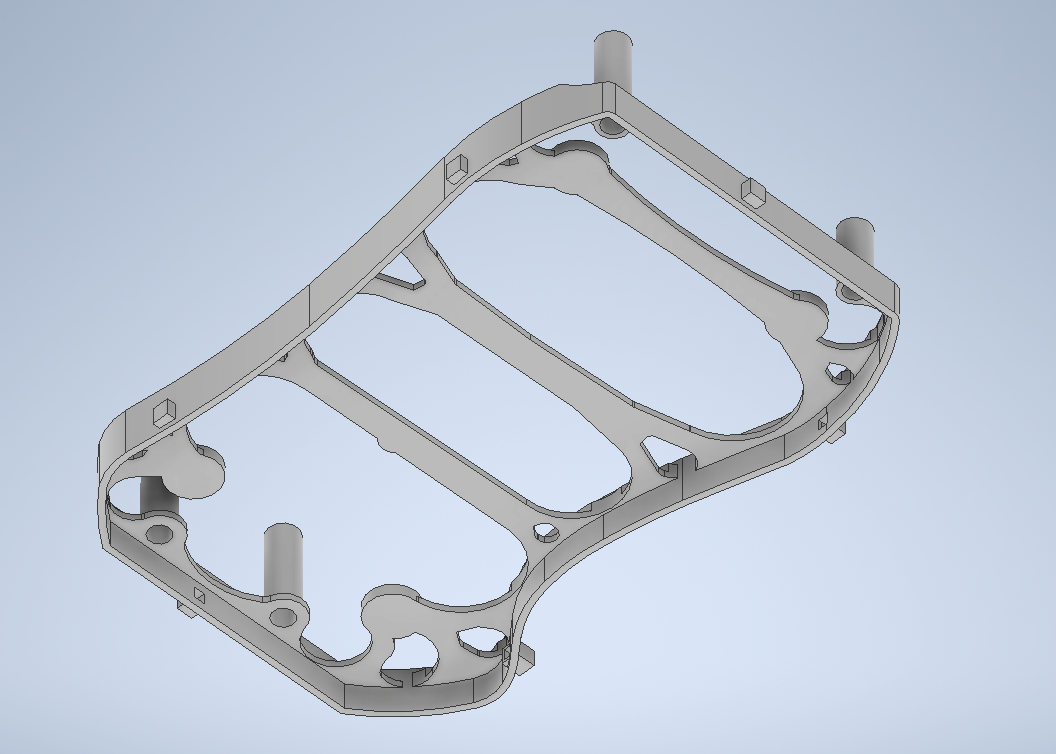
\includegraphics[width=\linewidth]{Bilder/Schuh_unten.png}
	\end{subfigure}
	\hfill
	\caption{}
	\label{Schuh_Inventor}
	%\vspace{0.1cm}
\end{figure}
% wesentliche Aufgabe des Schuhs
% Stabiler Ersatz der vorherigen Sohle -> hält nur mit den Schrauben
% Druckverteilung auf die Sensoren 
% Einsparung von Material in der Mitte
% Anpassung an den oberen Teil durch Auflage und Umfassung
% Einfassung des MAPs
% Basiert auf dem Scan des zweiteiligen Fußes von NAO.
% 4 Schrauben befestigen den unteren Teil an das obere Teil. Der Schuh ersetzt die eigentliche Sohle
% Das Gewicht des Roboters lastet hauptsächlich auf den 4 Drucksensoren, welche in Kap (Theorie) bereits erklärt wurden. Die 4 kreisförmigen Flächen liegen deshalb genau da an, wo diese Sensoren auch in dem ursprünglichen Teil anlagen. 
% Shape generater tragende Oberfläche.

\subsection{Herstellung des MAP} \FloatBarrier
\begin{figure}[tb]
	\hfill
	%\centering
	\begin{subfigure}[c]{.49\linewidth}
		\centering
		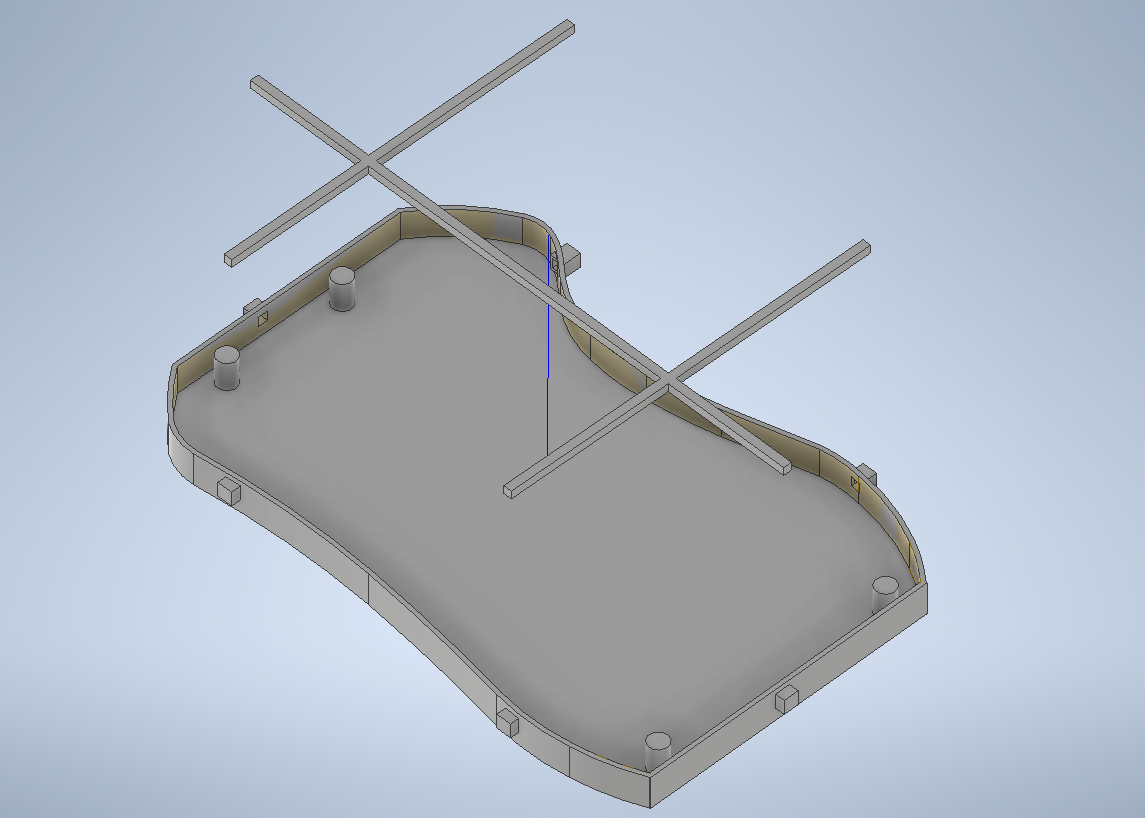
\includegraphics[width=\linewidth]{Bilder/Gussform_Innenteil_verschoben.png}
	\end{subfigure}
	\begin{subfigure}[c]{.49\linewidth}
		\centering
		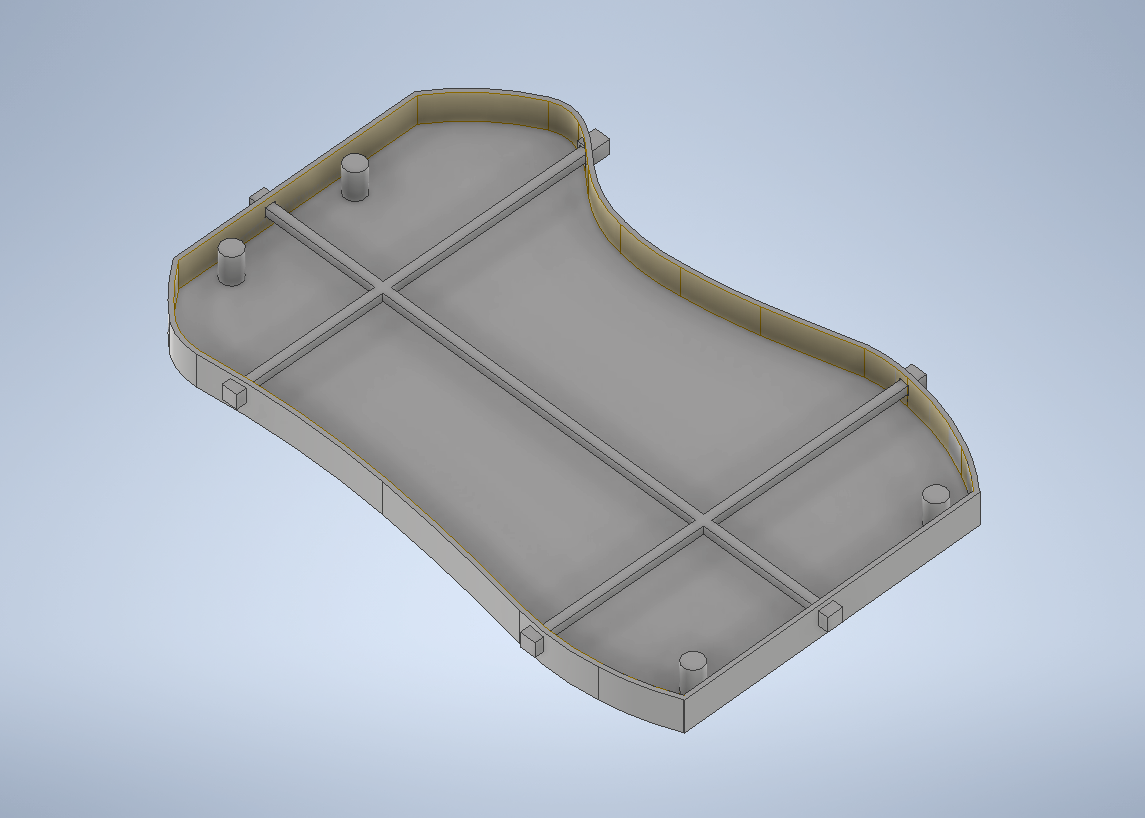
\includegraphics[width=\linewidth]{Bilder/Gussform.png}		
	\end{subfigure}
	\hfill
	\caption{Gussform der MAP Sohlen. Links ist die Innenhalterung herausgenommen, rechts ist sie eingespannt in den sechs Eckhalterungen.}
	\label{Gussform_Inventor}
	%\vspace{0.1cm}
\end{figure}
Das verwendete Polymer als Grundlage für das MAP ist ein additiv vernetzendes Silikon von (Firma und cite einbinden). Während dem Mischverfahren ist es flüssig und muss deshalb in eine Form gegeben werden. Silikon selbst lässt sich nur sehr schlecht durch etwaige Klebstoffe nach der Vernetzung verkleben. Deshalb wird hier wie in Abb. \ref{Gussform_Inventor} zu sehen ist, eine $2\unit{mm}$ dicke Stangenkonstruktion eingehängt, welche bis auf die 6 Enden mit MAP umschlossen wird. Diese, aus PLA gedruckte Konstrukt ist flexibel und kann deshalb durch Verbiegen in die Verankerungen gedrückt werden. Nach der vollständigen Vernetzung kann die Sohle aus der Form entnommen und in den Schuh aus dem vorherigen Kapitel eingesetzt werden. 

Die vier Zylinder dienen einem Platzhalter um die sechs Ecken in der Halterung des Schuhs für einen besseren Halt festzukleben und dann durch die Löcher des MAPs die Schrauben lockern zu können. 

\subsection{Laufstegkonstruktion} \FloatBarrier
Der NAO Roboter ist für den Einsatz auf geraden Bodenflächen im Innenbereich ausgelegt wobei er bei einem Bewegungsablauf ohne Anpassung an die Umwelt wie mit dem Befehl \texttt{moveTo()} durch Rutschen nicht immer die gleiche Strecke zurücklegt. 
Um wiederholbare Messreihen garantieren zu können ist eine Teststrecke von Nöten. Desweiteren sind verschiedene, flache Untergründe für eine Sohlenentwicklung interessant.
Außerdem kann auf das MAP nur Einfluss genommen werden, wenn ein magnetisches Feld angelegt wird. Deshalb muss wurde ein Laufsteg mit einem Hohlraum angefertigt, um unter der Fläche, auf der NAO läuft, Magneten angebracht werden. 

\begin{figure}[tb]
	\hfill
	%\centering
	\begin{subfigure}[c]{.49\linewidth}
		\centering
		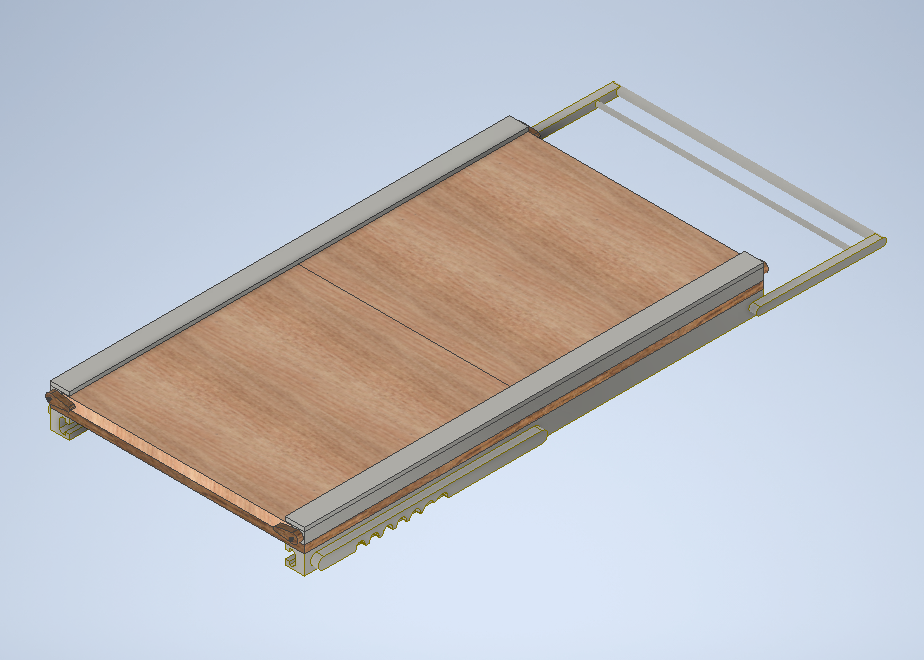
\includegraphics[width=\linewidth]{Bilder/Rampe_oben.png}
	\end{subfigure}
	\begin{subfigure}[c]{.49\linewidth}
		\centering
		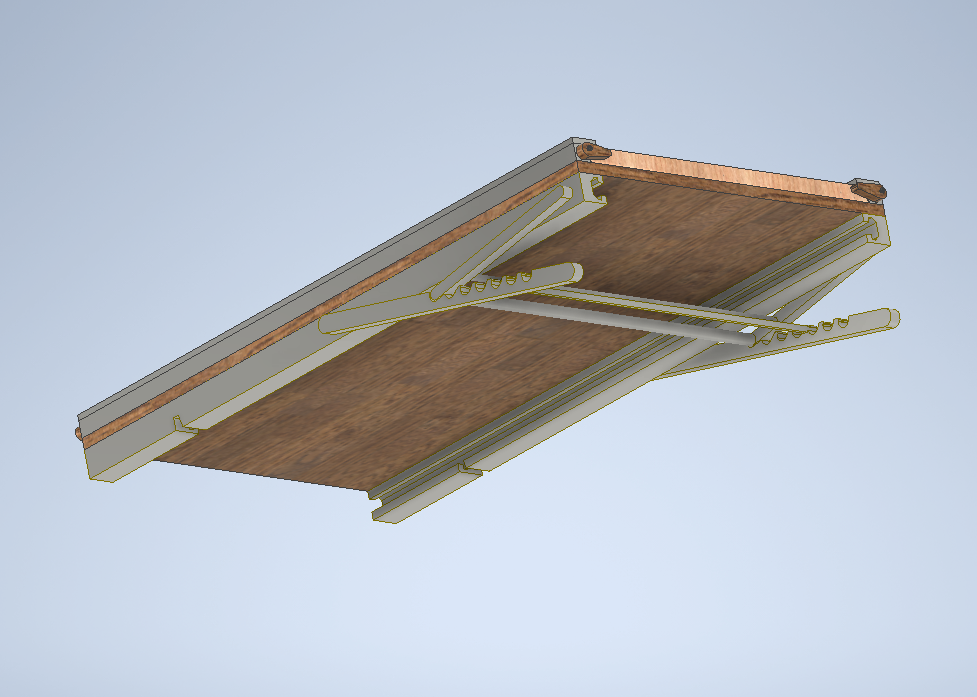
\includegraphics[width=\linewidth]{Bilder/Rampe_unten.png}
	\end{subfigure}
	\hfill
	\caption{Laufstegrampenkonstruktion mit zwei austauschbaren Platten und einer Winkelverstellung mit Raste. Links: Sicht von schräg oben mit eingeklappter Winkelverstellung. Rechts: Sicht von schräg unten mit niedigster Winkeleinstellung.}
	\label{Rampe_Inventor}
	%\vspace{0.1cm}
\end{figure}
\begin{wrapfigure}{hr}{0.4\linewidth}
	\vspace{-0.5cm}
	\centering
	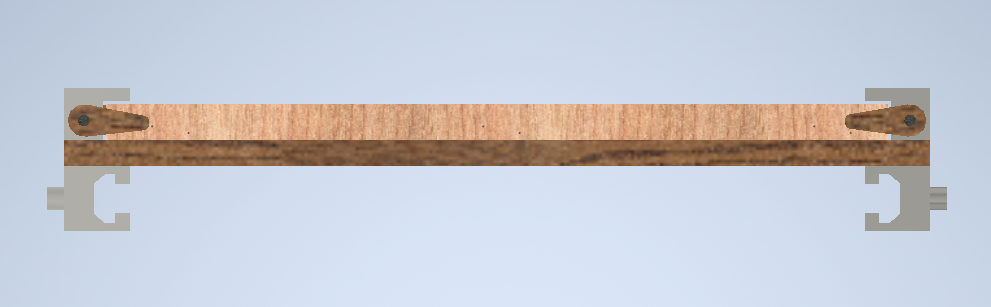
\includegraphics[width=\linewidth]{Bilder/Rampe_Seitenansicht3.png}
	\caption{Seitenansicht der Rampe mit einer Breite von $66,4 \unit{cm}$.}
	\label{Rampe_Seite_Inventor}
	\vspace{-0.5cm}
\end{wrapfigure}
% Aufbau der Rampe
Der Laufsteg besteht aus einer $120\times66,4 \unit{cm}$ großen Pressholzplatte, die auf der Oberseite mit einem Aluminiumkonstrukt erweitert ist, welches die Einschubplatten von beiden Längsseiten und nach oben hin abschließt, Abb. \ref{Rampe_Inventor} links. Auf den kurzen Seiten verriegeln jeweils Zwei drehbare Keile den Einschub, sodass die Platten eingeschlossen werden, Abb. \ref{Rampe_Seite_Inventor}.

Auf der Unterseite sind an den Längsseiten zwei mit T-Nut versehene Aluminumstangen angebracht, sowie eine zweiteilige Stangenkonstruktion, die eine Winkelverstellung mit Raste erlaubt, zu sehen in Abb. \ref{Rampe_Inventor} rechts. Die einstellbaren Winkel betragen ca. $5^\circ$ bis $17^\circ$, oder es wird für $0^\circ$ vollständig eingeklappt.
  

Man hat bereits NAO schräge Flächen gehen lassen wie in (cite). Dies erfordert einen komplett anderen Gang und hätte den Rahmen dieser Arbeit gesprengt. Die Neodymmagnete, die verwendet wurden, haben eine Haftkraft von ca. $16 \unit{kg}$, eine Maße von $40\times40\times4 \unit{mm}$ \cite{schraubmagnet} und wurden an die Unterseite der Rampe geschraubt. Die ersten Versuche ergaben schließlich, dass das MAP nur bei einem Abstand unter den Einlageplatten reagierte. Deshalb wurde in den hiesigen Messungen nur ohne Platten gemessen.


% Was man für die Messungen verwendet hat

%\subsubsection{Genaueres zum Einsatz an dem Nao Roboter}

%%% Local Variables:
%%% mode: latex
%%% TeX-master: "main"
%%% End: